\documentclass[a4paper,10pt]{exam}
\usepackage{graphicx}
\usepackage[document]{ragged2e}
 \usepackage[margin=1in]{geometry}
\usepackage{circuitikz}
\usepackage{tikz}
\usetikzlibrary{arrows.meta, shapes, circuits.ee.IEC, positioning}
\usepackage{float}
\usepackage{amsmath}
\usepackage{multicol}
\usepackage{enumitem}
\usepackage{setspace}
\usepackage{amssymb}

\usepackage{cite}
\usepackage{graphicx}
\usepackage{amsmath,amssymb,amsfonts,amsthm}
\usepackage{algorithmic}
\usepackage{graphicx}
\usepackage{textcomp}
\usepackage{xcolor}
\usepackage{txfonts}
\usepackage{listings}
\usepackage{enumitem}
\usepackage{mathtools}
\usepackage{gensymb}
\usepackage{comment}
\usepackage[breaklinks=true]{hyperref}
\usepackage{tkz-euclide} 
\usepackage{listings}
\usepackage{gvv}                                        
%\def\inputGnumericTable{}                                 
\usetikzlibrary{arrows.meta, positioning}
\usepackage{xparse}
\usepackage{color}                                            
\usepackage{array}                                            
\usepackage{longtable}                                       
\usepackage{calc}                                             
\usepackage{multirow}
\usepackage{multicol}
\usepackage{hhline}                                           
\usepackage{ifthen}                                           
\usepackage{lscape}
\usepackage{tabularx}
\usepackage{array}
\usepackage{float}
\newtheorem{theorem}{Theorem}[section]
\newtheorem{problem}{Problem}
\newtheorem{proposition}{Proposition}[section]
\newtheorem{lemma}{Lemma}[section]
\newtheorem{corollary}[theorem]{Corollary}
\newtheorem{example}{Example}[section]
\newtheorem{definition}[problem]{Definition}
\newcommand{\BEQA}{\begin{eqnarray}}
\newcommand{\EEQA}{\end{eqnarray}}
\usepackage{float}
%\newcommand{\define}{\stackrel{\triangle}{=}}
\theoremstyle{remark}
\usepackage{circuitikz}
\usepackage{tikz}
\usepackage{ragged2e}


\begin{document}
\begin{center}
\textbf{2007\\EE:Electrical Engineering}
\end{center}
\vspace{0.5cm}
\raggedright{Duration:Three hours}
\hfill
\raggedleft{Maximum Marks :150}
\vspace{0.98mm}
\begin{center}
    \textbf{Read the following instructions carefully.}
\end{center}
\begin{enumerate}
 \item This question paper contains 85 objective type questions. Q.1 to Q.20 carry \textbf{one mark} each and Q.21 to Q.85 carry \textbf{two marks} each.
\item Attempt all the questions.
    
    \item Questions must be answered on \textbf{Objective Response Sheet (ORS)} by darkening the appropriate bubble (marked A, B, C, D) using HB pencil against the question number on the left-hand side of the \textbf{ORS}. \textbf{Each question has only one correct answer.} In case you wish to change an answer, erase the old answer completely.
    
    \item Wrong answers will carry \textbf{NEGATIVE} marks. In Q.1 to Q.20, \textbf{0.25} mark will be deducted for each wrong answer. In Q.21 to Q.76, Q.76, Q.78, Q.80, Q.82 and in Q.84, \textbf{0.5} mark will be deducted for each wrong answer. However, there is no negative marking in Q.77, Q.79, Q.81, Q.83 and in Q.85. More than one answer bubbled against a question will be taken as an incorrect response. Unattempted questions will not carry any marks.
    
    \item Write your registration number, your name and name of the examination centre at the specified locations on the right half of the \textbf{ORS}.
    
    \item Using HB pencil, darken the appropriate bubble under each digit of your registration number and the letters corresponding to your paper code.
    
    \item Calculator is allowed in the examination hall.
    
    \item Charts, graph sheets or tables are \textbf{NOT} allowed in the examination hall.
    
    \item Rough work can be done on the question paper itself. Additionally blank pages are given at the end of the question paper for rough work.
    
    \item This question paper contains \textbf{32} printed pages including pages for rough work. Please check all pages and report, if there is any discrepancy.
\end{enumerate}
\vfill
\raggedright{\textbf{S/121 Food/06--EE--1A}}\\
\centering{EE 1/32}
\newpage
\begin{center}
    \textbf{Q.1 – Q.20 carry one mark each.}
\end{center}
\vspace{1em}
\begin{enumerate}
   

\item   The common emitter forward current gain of the transistor shown is $\beta_F = 100 $  \hfill{(GATE EE 2007)} 

\begin{figure}[H]
    \centering
    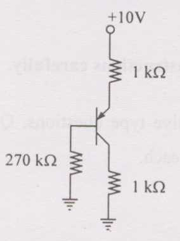
\includegraphics[width=0.4\linewidth]{figs/Q1.png} \caption{}     \label{fig:myfigure}
   
\end{figure}

\raggedright{The transistor is operating in}
\begin{multicols}{2}
\begin{enumerate}
\item Saturation region
\item Cutoff region
\item Reverse active region
\item Forward active region
\end{enumerate}
\end{multicols}
\vspace{0.5cm}
\item   The three-terminal linear voltage regulator is connected to a 10\( \Omega \)
 load resistor as shown in the figure. If \( V_{in} \)
 is 10 V, what is the power dissipated in the transistor?\hfill{(GATE EE 2007)} 
\begin{figure}[H]
    \centering
    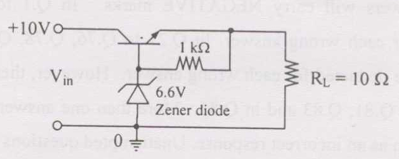
\includegraphics[width=0.5\linewidth]{figs/Q 2.png} \caption{}     \label{fig:myfigure}
   
\end{figure}
\begin{multicols}{4}
\begin{enumerate}
\item 0.6 W
\item 2.4 W
\item 4.2 W
\item 5.4 W
\end{enumerate}
\end{multicols}
\vfill
\centering{EE 2/32}\\

\raggedleft{\textbf{S/121 Food/06--EE--1B}}\\
\newpage
\item 
Consider the transformer connections in a part of a power system shown in the figure. The nature of transformer connections and phase shifts are indicated for all but one transformer.\\

Which of the following connections, and the corresponding phase shift $ \theta $
, should be used for the transformer between A and B?\hfill{(GATE EE 2007)} 
\begin{figure}[!ht]
\centering
\resizebox{0.7\textwidth}{!}{%
\begin{circuitikz}
\tikzstyle{every node}=[font=\small]
\draw (1.25,12.25) to[short] (1.25,10.75);
\draw (0.75,11.5) to[short] (2.75,11.5);
\draw (2.25,11.5) to[short] (2.25,11);
\draw (2.25,11) to[short] (4,11);
\draw (4,11) to[short] (4,11.75);
\draw  (4,12) circle (0.25cm);
\draw  (4,12.25) circle (0.25cm);
\draw [short] (4,13) -- (4,12.5);
\draw [short] (3.75,13) -- (7,13);
\draw [short] (7,13) -- (7.5,13);
\draw [short] (7,13) -- (7,12);
\draw  (7,11.5) circle (0.25cm);
\draw  (7,11.75) circle (0.25cm);
\draw  (1.25,10.25) circle (0.25cm);
\draw  (1.25,10.5) circle (0.25cm);
\draw [short] (1.25,10) -- (1.25,9.25);
\draw [short] (0.5,9.25) -- (2.25,9.25);
\draw [short] (0.75,9.25) -- (0.75,8.75);
\draw [short] (1.75,9.25) -- (1.75,9);
\draw [short] (1.75,9) -- (3.25,9);
\draw [short] (3.25,9) .. controls (3.75,9.25) and (3.75,9.5) .. (4,9.5);
\draw  (4,9.25) circle (0.25cm);
\draw [short] (4.25,9.25) -- (5.5,9.25);
\draw [short] (5.5,9.25) -- (5.5,9.5);
\draw [short] (5,9.5) -- (7.75,9.5);
\draw [short] (7,11.25) -- (7,9.5);
\draw [short] (6.25,9.5) -- (6.25,8.75);
\draw [short] (1.75,10.75) -- (1.5,10.75);
\draw [short] (1.5,10.75) -- (1.75,11);
\draw [short] (1.75,10.75) -- (2,10.75);
\draw [short] (1.75,11) -- (2,10.75);
\draw [short] (4.5,11.75) -- (4.25,11.75);
\draw [short] (4.25,11.75) -- (4.5,12);
\draw [short] (4.5,11.75) -- (4.75,11.75);
\draw [short] (4.5,12) -- (4.75,11.75);
\draw [short] (4.75,8.5) -- (4.75,8.75);
\draw [short] (4.75,8.75) -- (5,9);
\draw [short] (4.75,8.75) -- (4.5,9);
\draw [short] (1.75,9.75) -- (1.75,10);
\draw [short] (1.75,10) -- (2,10.25);
\draw [short] (1.75,10) -- (1.5,10.25);
\draw (0.75,12.5) to[sinusoidal voltage source, sources/symbol/rotate=auto] (1.5,12.5);
\draw [->, >=Stealth] (6.75,12) .. controls (6.5,12) and (6.25,11.75) .. (6.75,11.25) ;
\draw [->, >=Stealth] (3.75,12.5) .. controls (3.5,12.5) and (3.25,12.25) .. (3.75,11.75) ;
\draw [->, >=Stealth] (0.75,10.75) .. controls (0.5,10.75) and (0.25,10.5) .. (0.75,10) ;
\draw [->, >=Stealth] (3.5,9.5) .. controls (3.75,10) and (4,10) .. (4.5,9.5) ;
\node [font=\small] at (6.5,11) {$\Theta$};
\node [font=\small] at (7.25,12.25) {A};
\node [font=\small] at (7.25,11) {B};
\node [font=\small] at (7.25,9) {220kV};
\node [font=\small] at (-0.25,8.75) {400kV};
\node [font=\small] at (0.25,11.75) {15kV};
\node [font=\small] at (3.25,12) {-30$\circ$};
\node [font=\small] at (4,10) {0$\circ$};
\node [font=\small] at (0.25,10.25) {30$\circ$};
\node [font=\normalsize] at (3.5,8.25) {Autotransformer};
\end{circuitikz}
}%
\caption{}
    \label{fig:myfigure}
\end{figure}

\begin{multicols}{2}
\begin{enumerate}
\item  Star - Star ($ \theta = 0^\circ$)
  \item Star - Delta($ \theta = -30^\circ $)
  \item  Delta - Star($ \theta = 30^\circ $)
    \item  Star - Zigzag($ \theta = 30^\circ $)
\end{enumerate}
\end{multicols}
\vspace{0.5cm}

\item  The incremental cost curves in Rs/MWhr for two generators supplying a common load of 700 MW are shown in the figures. The maximum and minimum generation limits are also indicated. The optimum generation schedule is:\hfill{(GATE EE 2007)} \\
\begin{figure}[!ht]
\centering
\resizebox{1.1\textwidth}{!}{%
\begin{circuitikz}
\tikzstyle{every node}=[font=\normalsize]
\draw [->, >=Stealth] (2.5,10.5) -- (2.5,14.75);
\draw [->, >=Stealth] (2.5,10.5) -- (8.75,10.5);
\draw [->, >=Stealth] (12.5,10.5) -- (12.5,14.75);
\draw [->, >=Stealth] (12.5,10.5) -- (18.75,10.5);
\draw [short] (4,12.25) -- (7.75,13);
\draw [short] (14.5,13.5) -- (18,14.25);
\draw [dashed] (4,12.25) -- (4,10.75);
\draw [dashed] (4,11) -- (4,10.5);
\draw [dashed] (7.75,13) -- (7.75,10.5);
\draw [dashed] (14.5,13.5) -- (14.5,10.5);
\draw [dashed] (18,14.25) -- (18,10.5);
\draw [dashed] (4,12.25) -- (2.5,12.25);
\draw [dashed] (7.75,13) -- (2.5,12.75);
\draw [dashed] (14.5,13.5) -- (12.5,13.5);
\draw [dashed] (18,14.25) -- (12.5,14);
\node [font=\small] at (2.25,12.75) {600};
\node [font=\small] at (2.25,12.25) {450};
\node [font=\small] at (12,14.25) {800};
\node [font=\small] at (12,13.5) {650};
\node [font=\normalsize] at (4,10.25) {200MW};
\node [font=\normalsize] at (7.75,10.25) {450MW};
\node [font=\normalsize] at (14.5,10.25) {150MW};
\node [font=\normalsize] at (18,10.25) {400MW};
\node [font=\normalsize] at (3.25,15.25) {Incremental Cost Rs/MWhr};
\node [font=\normalsize] at (13.75,15.25) {Incremental Cost Rs/MWhr};
\node [font=\normalsize] at (19.25,10.5) {P};
\node [font=\normalsize] at (9.25,10.5) {P};
\end{circuitikz}
}%
\caption{}
    \label{fig:myfigure}
\end{figure}
\hspace{0.5in} \textbf{GENERATOR A} \hspace{2in} \textbf{GENERATOR B}\\
\vspace{0.3cm}
\begin{enumerate}[label=(\Alph*)]
\item Generator A: 400 MW, Generator B: 300 MW
\item  Generator A: 350 MW, Generator B: 350 MW
\item Generator A: 450 MW, Generator B: 250 MW
\item Generator A: 425 MW, Generator B: 275 MW
\end{enumerate}
\vspace{0.5cm}
\centering{EE 3/32}
\newpage
\item  Two regional systems, each having several synchronous generators and loads are interconnected by an ac line and a HVDC link as shown in the figure. Which of the following statements is true in the steady state:\hfill{(GATE EE 2007)} 
\begin{figure}[!ht]
\centering
\resizebox{0.8\textwidth}{!}{%
\begin{circuitikz}
\tikzstyle{every node}=[font=\large]


\draw (1.5,11.25) ellipse (2.5cm and 3.5cm);
\draw (11.75,11.25) ellipse (2.5cm and 3.5cm);


\draw [short] (3,9.5) -- (10.25,9.5);
\draw [line width=0.5pt] (3,12.75) -- (4.5,12.75);
\draw [line width=0.5pt] (10.25,12.75) -- (8.5,12.75);
\draw [line width=0.5pt] (4.5,12.75) -- (4.75,12.75);


\draw [line width=0.5pt] (4.75,13.5) rectangle (6.25,12);
\draw [line width=0.5pt] (7,13.5) rectangle (8.5,12);


\draw [line width=0.5pt] (6.25,13) -- (7,13);


\draw [line width=0.5pt, ->, >=Stealth] (6,14.25) -- (7.25,14.25);
\draw [line width=0.5pt, ->, >=Stealth] (6.25,8.75) -- (7.5,8.75);


\draw [line width=0.5pt] (5.5,12.75) -- (5,12.25);
\draw [line width=0.5pt] (5,12.25) -- (5.75,12.25);
\draw [line width=0.5pt] (5.5,12.75) -- (5.75,12.25);
\draw [line width=0.5pt] (5,12.75) -- (5.75,12.75);
\draw [line width=0.5pt] (5.5,13.25) -- (5.5,12.75);
\draw [line width=0.5pt] (5.5,12.75) -- (5.75,13);


\draw [line width=0.5pt] (7.25,13.25) -- (8,13.25);
\draw [line width=0.5pt] (7.25,13.25) -- (7.75,12.75);
\draw [line width=0.5pt] (8,13.25) -- (7.75,12.75);
\draw [line width=0.5pt] (7.25,12.75) -- (8,12.75);
\draw [line width=0.5pt] (7.75,12.75) -- (7.75,12.25);
\draw [line width=0.5pt] (7.75,12.75) -- (8,12.5);


\node at (1.5,11.25) {Region 1};
\node at (12,11) {Region 2};
\node at (6.75,11.5) {HVDC link};
\node at (6.5,10) {AC line};
\node at (6.5,15) {$P_{dc}$};
\node at (7,8) {$P_{ac}$};

\end{circuitikz}
}%
\caption{}
    \label{fig:myfigure}
\end{figure}
\begin{enumerate}[label=(\Alph*)]
\item Both regions need not have the same frequency

\item The total power flow between the regions (\( P_{ac} \)
+\( P_{dc} \)
) can be changed by controlling the HVDC converters alone

\item The power sharing between the ac line and the HVDC link can be changed by controlling the HVDC converters alone.
\item  The direction of power flow in the HVDC link (P) cannot be reversed.
\end{enumerate}
\vspace{1cm}
\item  Consider a bundled conductor of an overhead line, consisting of three identical sub-conductors placed at the corners of an equilateral triangle as shown in the figure. If we neglect the charges on the other phase conductors and ground, and assume that spacing between sub-conductors is much larger than their radius, the maximum electric field intensity is experienced at\hfill{(GATE EE 2007)} 
\begin{figure}[!ht]
\centering
\resizebox{0.3\textwidth}{!}{%
\begin{circuitikz}
\tikzstyle{every node}=[font=\LARGE]
\draw  (9,14) circle (0.75cm);
\draw [ line width=0.5pt ] (6,8.5) circle (0.75cm);
\draw [ line width=0.5pt ] (12.75,8.5) circle (0.75cm);



\node [font=\normalsize] at (9,14.75) {\textbf{.}};
\node [font=\normalsize] at (9,13.25) {\textbf{.}};
\node [font=\normalsize] at (7.25,11) {\textbf{.}};
\node [font=\normalsize] at (9.25,10) {\textbf{.}};
\node [font=\LARGE] at (9.5,12.75) {\textbf{X}};
\node [font=\LARGE] at (9.25,15.25) {\textbf{Y}};
\node [font=\LARGE] at (7.75,11.5) {\textbf{Z}};
\node [font=\LARGE] at (10,10) {\textbf{W}};
\end{circuitikz}
}%
\caption{}
    \label{fig:myfigure}
\end{figure}
\begin{multicols}{4}
    \begin{enumerate}
        \item  Point X
        \item  Point Y
        \item  Point Z
        \item  Point W
    \end{enumerate}
\end{multicols}

\vfill
\centering{EE 4/32}
\newpage
\item  The circuit shown in the figure is \hfill{(GATE EE 2007)} 

\begin{figure}[!ht]
\hspace{4in}
\resizebox{0.4\textwidth}{!}{%
\begin{circuitikz}
\tikzstyle{every node}=[font=\huge]


\draw (1,18) to[battery2] (1,5);


\draw[line width=1.4pt] (1,18) -- (9.25,18);
\draw[line width=1.4pt] (9.25,18) to[european resistor] (9.25,12.75);
\draw[line width=1.4pt] (9.25,12.75) to[european resistor] (9.25,7.5);
\draw[line width=1.4pt] (0.75,5.25) -- (18,5.25);
\draw[line width=1.4pt] (9.25,7.75) -- (9.25,5.25);


\draw[line width=1pt] (9.25,13.75) -- (13,13.75);
\draw[line width=1pt] (13,14.75) -- (13,10.25);
\draw[line width=1pt] (13,14.75) -- (15.25,12.5);
\draw[line width=1pt] (13,10.25) -- (15.25,12.5);


\draw[line width=1pt] (13,11.75) -- (12,11.75);
\draw[line width=1pt] (12,11.75) -- (12,8.5);
\draw[line width=1pt] (12,8.5) -- (18,8.5);


\draw[line width=1pt] (15,12.5) -- (18,12.5);
\draw[line width=1pt] (17.75,12.5) to[european resistor] (17.75,8.5);
\draw[line width=1pt] (17.75,8.5) to[european resistor] (17.75,5.25);


\node[font=\LARGE] at (19.25,10.5) {LOAD};
\node[font=\huge] at (18.5,6.75) {$r$};
\node[font=\huge] at (8.5,15.75) {$R_1$};
\node[font=\huge] at (8.25,10) {$R_2$};
\node[font=\huge] at (-0.75,11.25) {$V$};
\node[font=\huge] at (0.5,12.25) {+};
\node[font=\huge] at (0.5,10.75) {-};
\node[font=\huge] at (13.5,13.5) {+};
\node[font=\huge] at (13.5,11.75) {-};

\end{circuitikz}
}%
\caption{}
    \label{fig:myfigure}
\end{figure}

\begin{enumerate}

\item a voltage source with voltage $ \frac{rV}{R_1 \parallel R_2}$
\item a voltage source with voltage 
$\frac{r \parallel R_2}{R_1} V$

\item a current source with current 
$\frac{ r \parallel R_2 }{R_1 + R_2} \cdot \frac{V}{r}$

\item  a current source with current$ \frac{R_2}{R_1 + R_2} \cdot \frac{V}{r}$

\end{enumerate}
\vspace{0.4cm}
\item The system shown in the figure is\hfill{(GATE EE 2007)} 
\begin{figure}[!ht]

\hspace{5in}

\resizebox{0.5\textwidth}{!}{%
\begin{circuitikz}
\tikzstyle{every node}=[font=\Large]
\draw [line width=0.8pt, ->, >=Stealth] (4.5,-5.75) -- (6,-5.75);
\draw [ line width=0.8pt ] (7,-5.75) circle (1cm);
\draw [line width=0.8pt, ->, >=Stealth] (8,-5.75) -- (9.75,-5.75);
\draw [ line width=0.8pt ] (9.75,-4.75) rectangle (13.25,-6.5);
\draw [line width=0.8pt, short] (13.25,-5.75) -- (15,-5.75);
\draw [line width=0.8pt, ->, >=Stealth] (15,-5.75) -- (15,-8);
\draw [ line width=0.8pt ] (15,-9) circle (1cm) node {\LARGE \textbf{$\sum$}} ;
\draw [line width=0.8pt, ->, >=Stealth] (17.5,-9) -- (16,-9);
\draw [line width=0.8pt, ->, >=Stealth] (14,-9) -- (12.75,-9);
\draw [ line width=0.8pt ] (12.75,-10) rectangle (9.5,-8);
\draw [line width=0.8pt, short] (9.5,-9) -- (6.75,-9);
\draw [line width=0.8pt, ->, >=Stealth] (6.75,-9) -- (6.75,-6.75);
\node [font=\LARGE] at (7,-5.75) {\textbf{$\sum$}};
\node [font=\Large] at (4.75,-5) {$u_1$};
\node [font=\LARGE] at (15.5,-7.75) {\textbf{+}};
\node [font=\LARGE] at (16.25,-9.5) {\textbf{+}};
\node [font=\LARGE] at (5.75,-5.25) {\textbf{+}};
\node [font=\LARGE] at (5.75,-6.25) {\textbf{-}};
\node [font=\large] at (11.25,-5.25) {\textbf{s - 1}};
\node [font=\large] at (11.25,-5.75) {\textbf{s + 2}};
\node [font=\large] at (11.25,-8.75) {\textbf{1}};
\node [font=\large] at (11.25,-9.25) {\textbf{s - 1}};
\node [font=\Large] at (17.25,-8.25) {$u_2$};
\draw [line width=0.8pt, short] (10.75,-5.5) -- (12,-5.5);
\draw [line width=0.8pt, short] (10.75,-9) -- (11.75,-9);
\end{circuitikz}
}%
\caption{}
    \label{fig:myfigure}
\end{figure}
\begin{enumerate}
\item stable
\item unstable
\item conditionally stable
\item stable for input \(u_{1}\),but unstable for input $u_{2}$
\end{enumerate}


\vspace{1cm}

\item  Let a signal $ a_1 \sin(\omega_1 t + \phi_1)$ be applied to a stable linear time-invariant system. Let the corresponding steady state output be represented as $ a_2 F(\omega_1 t + \phi_2) $. Then which of the following statements is true?\hfill{(GATE EE 2007)} 
\begin{enumerate}
\item  F is not necessarily a "sine" or "cosine" function but must be periodic with $\omega_1= \omega_2$
\item  F must be a "sine" or "cosine" function with $a_1=a_2$
\item  F must be a "sine" function with $\omega_1= \omega_2$ and   $\phi_1 = \phi_2$
\item  F must be a "sine" or "cosine" function with $\omega_1=\omega_2$
\end{enumerate}

\vspace{0.5cm}

\centering{EE 5/32}
\newpage

\item  The frequency spectrum of a signal is shown in the figure. If this signal is ideally sampled at intervals of 1 ms, then the frequency spectrum of the sampled signal will be\hfill{(GATE EE 2007)} 

\begin{figure}[H]
    \centering
    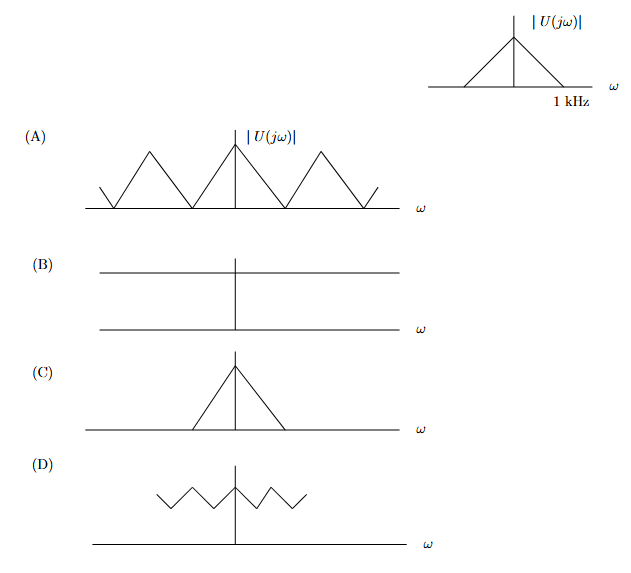
\includegraphics[width=0.75\linewidth]{figs/Q 10.png} \caption{}     \label{fig:myfigure}
    
\end{figure}

\item  Divergence of the vector field\hfill{(GATE EE 2007)} 
\begin{align}
\textbf{V}(x,y,z)=-(x cos xy+y)\textbf{i}+ 
(y \cos xy)\textbf{j}+(\sin z^2+x^2+y^2)\textbf{k} is        
\end{align}


\begin{multicols}{2}
\begin{enumerate}
\item $ 2z \cos z^{2}$
\item $\sin xy + 2z \cos z^{2}$
\item $ x \sin xy - \cos z$
\item none of these
\end{enumerate}
\end{multicols}
\vspace{0.5cm}

\noindent
\item  \quad $\vec{x} = [x_1\ x_2\ \ldots\ x_n]^{\mathrm{T}}$ is an $n$-tuple nonzero vector. The $n \times n$ matrix $V = \vec{x} \vec{x}^{\mathrm{T}}$ \hfill{(GATE EE 2007)} 

\begin{multicols}{2}
\begin{enumerate}
\item has rank zero
\item has rank 1
\item is orthogonal
\item has rank n
\end{enumerate}
\end{multicols}

\noindent
\item  \quad A single-phase fully controlled thyristor bridge ac-dc converter is operating at a firing angle of $25^\circ$ and an overlap angle of $10^\circ$ with constant dc output current of 20 A. The fundamental power factor (displacement factor) at input ac mains is \hfill{(GATE EE 2007)} 

\begin{multicols}{2}
\begin{enumerate}
 \item    0.78
\item  0.827
\item 0.866
\item  0.9
\end{enumerate}
\end{multicols}

\centering{EE 6/32}
\newpage

\item A three-phase, fully-controlled thyristor bridge converter is used as line commutated inverter to feed 50 kW power at 420 V dc to a three-phase, 415 V (line), 50 Hz ac mains. Consider dc link current to be constant. The rms current of the thyristor is \hfill{(GATE EE 2007)} 

\begin{multicols}{4}
\begin{enumerate}
 \item 119.05 A
\item  79.37 A
\item 68.73 A 
\item  39.68 A
\end{enumerate}
\end{multicols}

\item  In a transformer, zero voltage regulation at full load is \hfill{(GATE EE 2007)} 

\begin{multicols}{4}
\begin{enumerate}
 \item  not possible
\item   possible at unity power factor load 
\item  possible at leading power factor load 
\item  possible at lagging power factor load
\end{enumerate}
\end{multicols}

\item  The dc motor, which can provide zero speed regulation at full load without any controller, is \hfill{(GATE EE 2007)} 

\begin{multicols}{4}
\begin{enumerate}
 \item series
\item  shunt
\item cumulative compound
\item  differential compound
\end{enumerate}
\end{multicols}

\item  The probes of a non-isolated, two-channel oscilloscope are clipped to points A, B and C in the circuit of the adjacent figure. $V_{\text{in}}$ is a square wave of a suitable low frequency. \\
The display on Ch$_1$ and Ch$_2$ are as shown on the right. Then the ``Signal'' and ``Ground'' probes $S_1, G_1$ and $S_2, G_2$ of Ch$_1$ and Ch$_2$ respectively are connected to points:\hfill{(GATE EE 2007)} 

\begin{figure}[H]
    \centering
    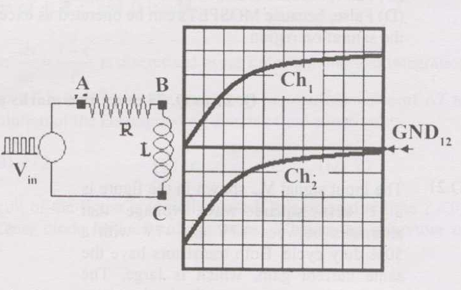
\includegraphics[width=0.6\linewidth]{figs/Q 17.png} \caption{}     \label{fig:myfigure}
   
\end{figure}

\begin{multicols}{4}
\begin{enumerate}
 \item  A,B,C,A
\item A,B,C,B
\item  C,B,A,B 
\item  B,A,B,C
\end{enumerate}
\end{multicols}

\item  A single phase full-wave half-controlled bridge converter feeds an inductive load. \\
The two SCRs in the converter are connected to a common DC bus. The converter has to have a freewheeling diode \hfill{(GATE EE 2007)} 
\begin{enumerate}
\item  because the converter inherently does not provide for free-wheeling
\item because the converter does not provide for free-wheeling for high values of triggering angles

\item  or else the free-wheeling action of the converter will cause shorting of the AC supply 
\item or else if a gate pulse to one of the SCRs is missed, it will subsequently cause a high load current in the other SCR
\end{enumerate}
\vfill
\centering{EE 7/32}
\newpage

\item  The electromagnetic torque $T_e$ of a drive, and its connected load torque $T_L$ are as shown below. Out of the operating points A, B, C and D, the stable ones are: \hfill{(GATE EE 2007)} 

\begin{figure}[!ht]
\centering
\resizebox{0.85\textwidth}{!}{%
\begin{circuitikz}
\tikzstyle{every node}=[font=\Large]

\draw [line width=1pt, ->, >=Stealth] (-1.5,-3.5) -- (-1.5,1.75);
\draw [line width=1pt, ->, >=Stealth] (-2,-3) -- (3.75,-3);

\draw [line width=1pt, ->, >=Stealth] (7.25,-3.5) -- (7.25,1.75);
\draw [line width=1pt, ->, >=Stealth] (6.75,-3) -- (12.5,-3);

\draw [line width=1pt, ->, >=Stealth] (16,-3.25) -- (16,2);
\draw [line width=1pt, ->, >=Stealth] (15.5,-2.75) -- (21.25,-2.75);

\draw [line width=1pt, ->, >=Stealth] (24.25,-3.25) -- (24.25,2);
\draw [line width=1pt, ->, >=Stealth] (23.75,-2.75) -- (29.5,-2.75);
\node at (-2.25,0.5) {T};
\node at (6.25,0.5) {T};
\node at (14.75,0.5) {T};
\node at (23.25,0.5) {T};

\node at (2.75,-3.75) {Speed};
\node at (11.5,-3.75) {Speed};
\node at (20.25,-3.5) {Speed};
\node at (28.5,-3.5) {Speed};

\draw [line width=1pt] (0.5,1.25) .. controls (1.5,2.75) and (1.75,-0.25) .. (3,-2);
\draw [line width=1pt] (0.5,-2) .. controls (2.25,-1.25) and (2.75,-0.75) .. (3.75,1);

\draw [line width=1pt] (8.25,-1.75) .. controls (9.5,0) and (11.25,3.25) .. (11.5,1.25);
\draw [line width=1pt] (7.75,-1) .. controls (9.75,-1) and (10.25,-0.25) .. (11,0.5);

\draw [line width=1pt] (16.5,-2) .. controls (17.75,-0.25) and (19.5,3) .. (19.75,1);
\draw [line width=1pt] (17,-2.25) .. controls (18.25,-1) and (18.25,0) .. (18.5,2.25);

\draw [line width=1pt] (26,1.5) .. controls (27,3.25) and (27.5,0) .. (28.75,-1.75);
\draw [line width=1pt] (26.25,1) .. controls (28.25,0.5) and (28.5,0) .. (29.25,-1.25);

\node at (0,1.75) {$T_e$};
\node at (10.25,2) {$T_e$};
\node at (20.25,1) {$T_e$};
\node at (27.25,2.5) {$T_e$};

\node at (4.25,1.25) {$T_L$};
\node at (11.25,-0.25) {$T_L$};
\node at (18.75,-0.5) {$T_L$};
\node at (29.75,-1) {$T_L$};


\node at (3,-1) {A};
\node at (9,-1.25) {B};
\node at (18,0.75) {C};
\node at (27.25,0.25) {D};

\end{circuitikz}
}%
\caption{}
    \label{fig:myfigure}
\end{figure}
\begin{multicols}{4}
\begin{enumerate}
 \item  A, C, D
\item B, C 
\item   A, D 
\item  B, C, D
\end{enumerate}
\end{multicols}

\item  ``Six MOSFETs connected in a bridge configuration (having no other power device), MUST be operated as a Voltage Source Inverter (VSI)''. This statement is: \hfill{(GATE EE 2007)} 
\begin{enumerate}
 \item  True, because being majority carrier devices, MOSFETs are voltage driven 
 \item  True, because MOSFETs have inherently anti-parallel diodes
 \item  False, because it can be operated both as Current Source Inverter (CSI) or a VSI 
 \item False, because MOSFETs can be operated as excellent constant current sources in the saturation region 
\end{enumerate}
\textbf{Q.21 to Q.75 carry two marks each.}\\[3ex]

\item  The input signal $V_{\text{in}}$ shown in the figure is a 1 kHz square wave voltage that alternates between +7V and -7V with a 50\% duty cycle. Both transistors have the same current gain, which is large. The circuit delivers power to the load resistor $R_L$. What is the efficiency of this circuit for the given input? Choose the closest answer. \hfill{(GATE EE 2007)} 

\begin{figure}[H]
    \centering
    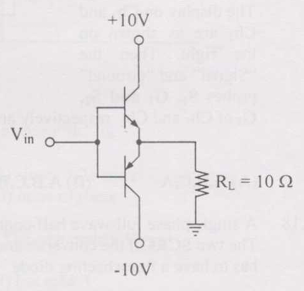
\includegraphics[width=0.5\linewidth]{figs/Q 21.png} \caption{}     \label{fig:myfigure}
    
\end{figure}

\begin{multicols}{4}
\begin{enumerate}
 \item 46\% 
\item 55\%
\item  63\% 
\item  92\% 
\end{enumerate}
\end{multicols}

\vfill
\centering{EE 8/32}
\newpage

\item  A, B, C and D are input bits, and Y is the output bit in the XOR gate circuit of the figure below. Which of the following statements about the sum S of A, B, C, D and Y is correct?\hfill{(GATE EE 2007)} 
\begin{figure}[!ht]
\centering
\resizebox{0.6\textwidth}{!}{%
\begin{circuitikz}
\tikzstyle{every node}=[font=\normalsize]
\draw (21.5,-12.5) to[short] (21.75,-12.5);
\draw (21.5,-13) to[short] (21.75,-13);
\draw (21.75,-12.5) node[ieeestd xor port, anchor=in 1, scale=0.89](port){} (port.out) to[short] (23.5,-12.75);
\draw [ line width=1pt](23.5,-12.75) to[short] (24.75,-12.75);
\draw [ line width=1pt](24.75,-12.75) to[short] (24.75,-13.5);
\draw [ line width=1pt](24.75,-13.5) to[short] (26.25,-13.5);
\draw (26.25,-13.5) to[short] (26.5,-13.5);
\draw (26.25,-14) to[short] (26.5,-14);
\draw (26.5,-13.5) node[ieeestd xor port, anchor=in 1, scale=0.89](port){} (port.out) to[short] (28.25,-13.75);
\draw (21.5,-14.5) to[short] (21.75,-14.5);
\draw (21.5,-15) to[short] (21.75,-15);
\draw (21.75,-14.5) node[ieeestd xor port, anchor=in 1, scale=0.89](port){} (port.out) to[short] (23.5,-14.75);
\draw [ line width=1pt](26.25,-14) to[short] (24.75,-14);
\draw [ line width=1pt](24.75,-14) to[short] (24.75,-14.75);
\draw [ line width=1pt](24.75,-14.75) to[short] (23.25,-14.75);
\node [font=\normalsize] at (27.25,-13.75) {$XOR$};
\node [font=\normalsize] at (22.5,-12.75) {$XOR$};
\node [font=\normalsize] at (22.5,-14.75) {$XOR$};
\node [font=\normalsize] at (21.25,-12.5) {$A$};
\node [font=\normalsize] at (21.25,-13) {$B$};
\node [font=\normalsize] at (21.25,-14.5) {$C$};
\node [font=\normalsize] at (21.25,-15) {$D$};
\node [font=\normalsize] at (28.5,-13.75) {$Y$};
\end{circuitikz}
}%
\caption{}
    \label{fig:myfigure}

\end{figure}
\begin{multicols}{4}
\begin{enumerate}
 \item S is always either zero or odd
\item S is always either zero or even
\item  s = 1 only if the sum of A, B, C and D is even 
\item s = 1 only if the sum of A, B, C and D is odd
\end{enumerate}
\end{multicols}
\vspace{0.5cm}
\item  The differential equation $\frac{dx}{dy}$ = $\frac{1-x}{\tau}$ is discretised using Euler's numerical integration method with a time step triangle $\Delta$T $>$  0 . What is the maximum permissible value of $\Delta$T to ensure stability of the solution of the corresponding discrete time equation?\hfill{(GATE EE 2007)} 
\begin{multicols}{4}
\begin{enumerate}
 \item 1
\item $\frac{\tau}{2}$
\item $\tau$
\item 2$\tau$
\end{enumerate}
\end{multicols}

\item  The switch S in the circuit of the figure is initially closed. It is opened at time t=0. You may neglect the Zener diode forward voltage drops. What is the behaviour of $V_{out}$ for t $>$ 0?\hfill{(GATE EE 2007)} 

\begin{figure}[H]
    \centering
    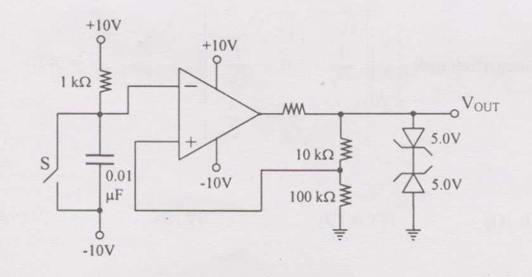
\includegraphics[width=0.5\linewidth]{figs/Q24 2007.png} 
   \caption{}
    \label{fig:myfigure}
\end{figure}

\begin{enumerate}
 \item  It makes a transition from -5 to +5 V at t= 12.98$\mu$s

 \item  It makes a transition from -5 to +5 V at t=2.57$\mu$s
 \item  It makes a transition from +5 to -5 V at t=12.98$\mu$s
 \item  It makes a transition from +5 to -5 V at t=2.57$\mu$s
\end{enumerate}
\vfill
\centering{EE 9/32}\\
\vspace{0.7cm}
\raggedright{\textbf{S/121 Food/06--EE--2A}}
\newpage
\item  A solid sphere made of insulating material has a radius R and has a total charge Q distributed uniformly in its volume. What is the magnitude of the electric field intensity, E, at a distance r(0 $<$ r $<$ R) inside the sphere?\hfill{(GATE EE 2007)} 
\begin{multicols}{4}
\begin{enumerate}
 \item $\frac{1}{4\pi\epsilon}$$\frac{Qr}{R^3}$
\item $\frac{3}{4\pi\epsilon}$$\frac{Qr}{R^3}$
\item $\frac{1}{4\pi\epsilon}$$\frac{Q}{r^3}$
\item $\frac{1}{4\pi\epsilon}$$\frac{QR}{r^3}$
\end{enumerate}
\end{multicols}

\item  The figure below shows a three phase self-commutated voltage source converter connected to a power system. The converter's de bus capacitor is marked as C in the figure. The circuit is initially operating in steady state with $\delta$= 0 and the capacitor de voltage is equal to \(V_{dc0}\). You may neglect all losses and harmonics. What action should be taken to increase the capacitor de voltage slowly to a new steady state value?\hfill{(GATE EE 2007)} 
\begin{figure}[!ht]
\centering
\resizebox{0.6\textwidth}{!}{%
\begin{circuitikz}
\tikzstyle{every node}=[font=\LARGE]
\draw (-1,11.75) to[short] (0.75,11.75);
\draw (-1,9.75) to[short] (0.75,9.75);
\draw  (0.75,13) rectangle (6.75,8.5);
\draw [short] (6.75,10.75) -- (8.25,10.75);
\draw [short] (10.5,10.75) -- (12,10.75);
\draw (12,10.75) to[sinusoidal voltage source, sources/symbol/rotate=auto] (12.75,10.75);
\draw (8.75,10) to[short] (7.75,9);
\draw (7.75,9) to[short] (8.75,9);
\draw (12.5,10) to[short] (11.5,9);
\draw (11.5,9) to[short] (12.75,9);
\node [font=\LARGE] at (-1.75,11) {C};
\node [font=\LARGE] at (5.75,9.25) {};
\node [font=\LARGE] at (11.5,9.5) {E};
\node [font=\LARGE] at (8.5,9.25) {$\delta$};
\node [font=\LARGE] at (12.25,9.25) {0};
\node [font=\LARGE] at (7.75,9.5) {E};
\draw [short] (8.25,10.75) .. controls (8.5,12) and (8.5,11.75) .. (9,10.75);
\draw [short] (9,10.75) .. controls (9.5,12) and (9.25,11.75) .. (9.75,10.75);
\draw [short] (9.75,10.75) .. controls (10.25,11.75) and (10,11.5) .. (10.5,10.75);
\draw [short] (-1,11.75) -- (-1,11);
\draw [short] (-1.5,11) -- (-0.5,11);
\draw [short] (-1.5,10.75) -- (-0.5,10.75);
\draw [short] (-1,10.75) -- (-1,9.75);
\node [font=\LARGE] at (3.75,11.25) {Three phase voltage};
\node [font=\LARGE] at (3.5,10.75) {source converter};
\end{circuitikz}
}%
\caption{}
    \label{fig:myfigure}
\end{figure}
\begin{enumerate}
\item Make $\delta$ positive and maintain it at a positive value
\item   Make $\delta$ positive and return it to its original value
\item  Make $\delta$ negative and maintain it at a negative value
\item Make $\delta$ negative and return it to its original value
\end{enumerate}
\vspace{1cm}
\item  The total reactance and total susceptance of a lossless overhead EHV line, operating at 50 Hz, are given by 0.045 pu and 1.2 pu respectively. If the velocity of wave propagation is 3 x $10^5$ km/s, then the approximate length of the line is\hfill{(GATE EE 2007)} 

\begin{multicols}{4}
\begin{enumerate}
 \item 122 km
\item 172km
\item 222km
\item 272km
\end{enumerate}
\end{multicols}
\vfill
\centering{EE 10/32}\\
\vspace{1cm}
\raggedleft{\textbf{S/121 Food/06--EE--2B}}
\newpage

\item  \quad
Consider the protection system shown in the figure below. The circuit breakers, numbered from 1 to 7 are of identical type. A single line to ground fault with zero fault impedance occurs at the midpoint of the line (at point F), but circuit breaker 4 fails to operate (\textquotedblleft stuck breaker\textquotedblright). If the relays are coordinated correctly, a valid sequence of circuit breaker operations is\hfill{(GATE EE 2007)} 

\begin{figure}[H]
    \centering
    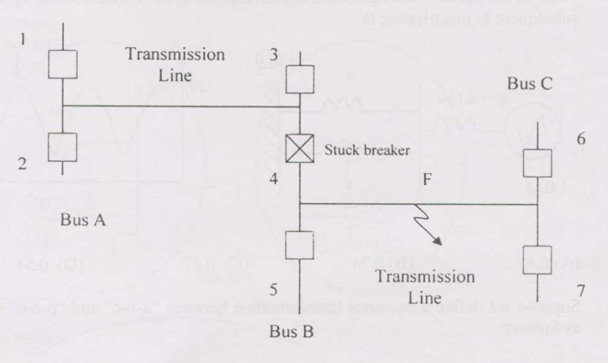
\includegraphics[width=0.75\linewidth]{figs/Q 28 2007.png} 
    \caption{}
    \label{fig:myfigure}
\end{figure}
\begin{multicols}{4}
\begin{enumerate}
 \item 1, 2, 6, 7, 3, 5 
\item  1, 2, 5, 6, 7, 3 
\item 5, 6, 7, 3, 1, 2 
\item 5, 1, 2, 3, 6, 7
\end{enumerate}
\end{multicols}

\item \quad
A three phase balanced star connected voltage source with frequency $\omega$ rad/s is connected to a star connected balanced load which is purely inductive. The instantaneous line currents and phase to neutral voltages are denoted by $(i_a, i_b, i_c)$ and $(v_{an}, v_{bn}, v_{cn})$ respectively, and their rms values are denoted by $V$ and $I$.\hfill{(GATE EE 2007)} 

$
\text{If}\ R = 
\myvec{
v_{an} & v_{bn} & v_{cn}
}
\myvec{
0 & \frac{1}{\sqrt{3}} & -\frac{1}{\sqrt{3}} \\
-\frac{1}{\sqrt{3}} & 0 & \frac{1}{\sqrt{3}} \\
\frac{1}{\sqrt{3}} & -\frac{1}{\sqrt{3}} & 0
}
\myvec{
i_a \\ i_b \\ i_c
},\ 
\text{then the magnitude of $R$ is}
$


\vspace{1cm}
\begin{multicols}{4}
\begin{enumerate}
\item  $3VI$
\item  $VI$
\item  $0.7VI$
\item  $0$
\end{enumerate}
\end{multicols}

\vfill
\centering{EE 11/32}
\newpage

\item  \quad
Consider a synchronous generator connected to an infinite bus by two identical parallel transmission lines. The transient reactance $x'$ of the generator is $0.1$ pu and the mechanical power input to it is constant at $1.0$ pu. Due to some previous disturbance, the rotor angle ($\delta$) is undergoing an undamped oscillation, with the maximum value of $\delta(t)$ equal to $130^\circ$. One of the parallel lines trips due to relay maloperation at an instant when $\delta(t) = 130^\circ$ as shown in the figure. The maximum value of the per unit line reactance, $x$, such that the system does not lose synchronism subsequent to this tripping is\hfill{(GATE EE 2007)} 

\begin{figure}[H]
    \centering
    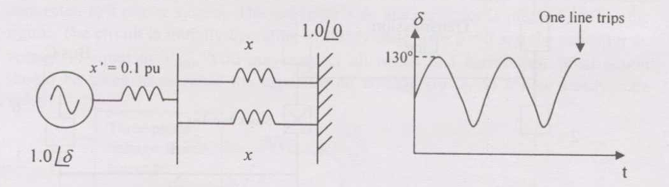
\includegraphics[width=0.7\linewidth]{figs/Q 30 2007.png} 
    \caption{}
    \label{fig:myfigure}
\end{figure}

\begin{multicols}{4}
\begin{enumerate}
\item  $0.87$
\item  $0.74$
\item  $0.67$
\item  $0.54$
\end{enumerate}
\end{multicols}

\item  \quad
Suppose we define a sequence transformation between ``a-b-c'' and ``p-n-o'' variables as follows:

$
\myvec{
f_a \\ f_b \\ f_c
}
=
k
\myvec{
1 & 1 & 1 \\ 
\alpha^2 & \alpha & 1 \\ 
\alpha & \alpha^2 & 1
}
\myvec{
f_p \\ f_n \\ f_o
}
\quad
\text{where } \alpha = e^{j\frac{2\pi}{3}} \text{ and $k$ is a constant.}
$

Now, if it is given that:

$
\myvec{ V_p \\ V_n \\ V_o } = 
\myvec{ 
0.5 & 0 & 0 \\
0 & 0.5 & 0 \\
0 & 0 & 2.0
}
\myvec{ i_p \\ i_n \\ i_o }
\text{ and }
\myvec{ V_a \\ V_b \\ V_c } = 
\myvec{ i_a \\ i_b \\ i_c }
$
then,\hfill{(GATE EE 2007)} 

\begin{multicols}{2}
\begin{enumerate}
\item  $Z = 
\myvec{ 
1.0 & 0.5 & 0.75 \\
0.75 & 1.0 & 0.5 \\
0.5 & 0.75 & 1.0 \\
}$ 

\item  $Z = 
\myvec{ 
1.0 & 0.5 & 0.5 \\
0.5 & 1.0 & 0.5 \\
0.5 & 0.5 & 1.0 \\
}$ 

\item  $Z = 3k^2
\myvec{ 
1.0 & 0.75 & 0.5 \\
0.5 & 1.0 & 0.75 \\
0.75 & 0.5 & 1.0 \\
}$ 

\item  $Z = \dfrac{k^2}{3}
\myvec{ 
1.0 & -0.5 & -0.5 \\
-0.5 & 1.0 & -0.5 \\
-0.5 & -0.5 & 1.0 \\
}$ 
\end{enumerate}
\end{multicols}


\vfill
\centering{EE 12/32}
\newpage

\item  \quad
Consider the two power systems shown in figure A below, which are initially not interconnected, and are operating in steady state at the same frequency. Separate loadflow solutions are computed individually for the two systems, corresponding to this scenario. The bus voltage phasors so obtained are indicated on figure A. These two isolated systems are now interconnected by a short transmission line as shown in figure B, and it is found that  $P_{1}$=  $P_{2}$ =  $Q_{1}$ =  $Q_{2}$ =0.\hfill{(GATE EE 2007)} 

\begin{figure}[H]
    \centering
    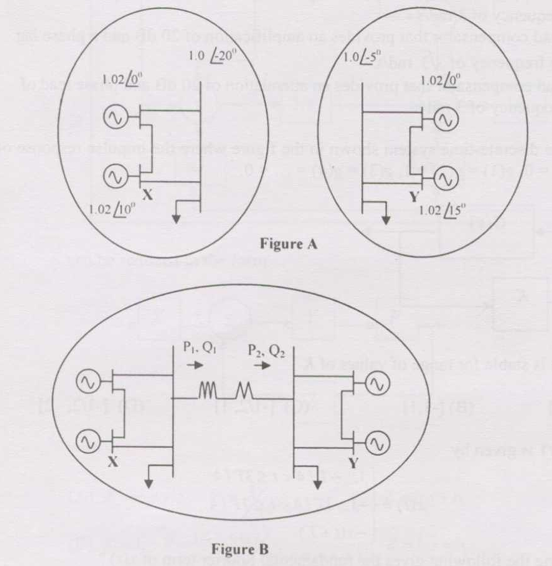
\includegraphics[width=0.6\linewidth]{figs/Q 32 2007.png} 
    \caption{}
    \label{fig:myfigure}
\end{figure}

The bus voltage phase angular difference between generator bus X and generator bus Y after the interconnection is

\begin{multicols}{4}
\begin{enumerate}
    \item  $10^{0}$
    \item  $25^{0}$
    \item  $-30^{0}$
    \item  $30^{0}$
    \end{enumerate}
\end{multicols}


\item  \quad The octal equivalent of the HEX number \textbf{AB.CD} is\hfill{(GATE EE 2007)} 

\begin{center}
\begin{multicols}{4}
\begin{enumerate}
\item  253.314
\item  253.632
\item  526.314
\item  526.632
\end{enumerate}
\end{multicols}
\end{center}

\item  \quad If $x = \text{Re}\ G(j\omega)$, and $y = \text{Im}\ G(j\omega)$ then for $\omega \to 0^{+}$, the Nyquist plot for\\
$G(s) = \dfrac{1}{s(s+1)(s+2)}$ becomes asymptotic to the line\hfill{(GATE EE 2007)} 

\begin{multicols}{4}
\begin{enumerate}
\item  $x = 0$
\item  $x = -3/4$
\item  $x = y - 1/6$
\item  $x = y/\sqrt{3}$
\end{enumerate}
\end{multicols}


\vfill
\centering{EE 13/32}
\newpage

\item  \quad The system $\dfrac{900}{s(s+1)(s+9)}$ is to be compensated such that its gain-crossover frequency becomes same as its uncompensated phase-crossover frequency and provides a $45^{0}$ phase margin. To achieve this, one may use\hfill{(GATE EE 2007)} 

\begin{enumerate}
    \item a lag compensator that provides an attenuation of 20 dB and a phase lag of $45^{0}$ at the frequency of $3\sqrt{3}$ rad/s
    \item a lead compensator that provides an amplification of 20 dB and a phase lead of $45^{0}$ at the frequency of 3 rad/s
    \item a lag-lead compensator that provides an amplification of 20 dB and a phase lag of $45^{0}$ at the frequency of $\sqrt{3}$ rad/s
    \item a lag-lead compensator that provides an attenuation of 20 dB and phase lead of $45^{0}$ at the frequency of 3 rad/s
\end{enumerate}

\item  \quad Consider the discrete-time system shown in the figure where the impulse response $G(z)$ is $g(0) = 0$, $g(1) = g(2) = 1$, $g(3) = g(4) = \cdots = 0$. \hfill{(GATE EE 2007)} 

\begin{figure}[H]
    \centering
    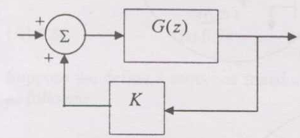
\includegraphics[width=0.4\linewidth]{figs/q 36 2007.png} 
\caption{}
    \label{fig:myfigure}
\end{figure}

This system is stable for range of values of $K$

\begin{multicols}{4}
\begin{enumerate}
\item  $[-1, 1/2]$
\item  $[-1, 1]$=
\item  $[-1/2, 1]$
\item  $[-1/2, 2]$
\end{enumerate}
\end{multicols}

\item A signal $x(t)$ is given by
$
x(t) = \begin{cases} 
1, & -\dfrac{T}{4} < t \leq \dfrac{3T}{4} \\\\ 
-1, & \dfrac{3T}{4} < t \leq \dfrac{7T}{4} \\\\ 
-x(t+T)
\end{cases}
$

Which among the following gives the fundamental Fourier term of $x(t)$?\hfill{(GATE EE 2007)} 

\begin{multicols}{2}
\begin{enumerate}

\item  $\dfrac{4}{\pi} \cos\left(\dfrac{\pi t}{T} - \dfrac{\pi}{4}\right)$

\item  $\dfrac{\pi}{4} \cos\left(\dfrac{\pi t}{2T} + \dfrac{\pi}{4}\right)$

\item  $\dfrac{4}{\pi} \sin\left(\dfrac{\pi t}{T} - \dfrac{\pi}{4}\right)$

\item  $\dfrac{\pi}{4} \sin\left(\dfrac{\pi t}{2T} + \dfrac{\pi}{4}\right)$
\end{enumerate}
\end{multicols}



\item  If the loop gain $K$ of a negative feedback system having a loop transfer function $\dfrac{K(s+3)}{(s+8)^2}$ is to be adjusted to induce a sustained oscillation then\hfill{(GATE EE 2007)} 

\begin{enumerate}
    \item The frequency of this oscillation must be $\dfrac{4}{\sqrt{3}}$ rad/s
    \item The frequency of this oscillation must be 4 rad/s
    \item The frequency of this oscillation must be 4 or $\dfrac{4}{\sqrt{3}}$ rad/s
    \item such a $K$ does not exist
\end{enumerate}
\centering{EE 14/32}
\newpage
\item   The system shown in figure below\hfill{(GATE EE 2007)} 

\begin{figure}[H]
    \centering
    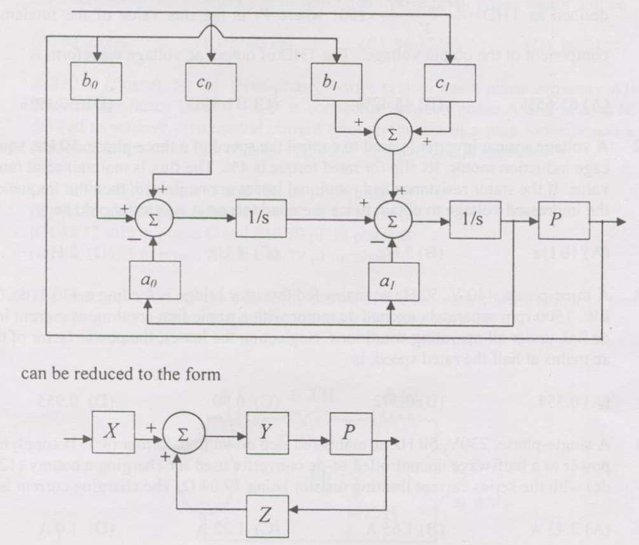
\includegraphics[width=0.75\linewidth]{figs/Q 39 2007.png} 
    \caption{}
    \label{fig:myfigure}
\end{figure}

with

\begin{enumerate}
   \item $X = c_0 s + c_1,$ \quad $Y = \dfrac{1}{s^{2} + a_0 s + a_1},$\quad $Z = b_0 s + b_1$

\item $X = 1,$ \quad $Y = \dfrac{c_0 s + c_1}{s^2 + a_0 s + a_1},$\quad $Z = b_0 s + b_1$

\item $X = c_1 s + c_0,$ \quad $Y = \dfrac{b_1 s + b_0}{s^2 + a_1 s + a_0},$\quad $Z = 1$

\item $X = c_1 s + c_0,$ \quad $Y = \dfrac{1}{s^2 + a_1 s + a_0},$\quad $Z = b_1 s + b_0$
\end{enumerate}
\item  \quad
The value of 
$
\oint_C \frac{dz}{1 + z^2}
$
where $C$ is the contour $|z - i/2| = 1$ is\hfill{(GATE EE 2007)} 
\begin{multicols}{4}
\begin{enumerate}
\item  $2\pi i$
\item  $\pi$
\item  $\tan^{-1} z$
\item $\pi i \tan^{-1} z$
\end{enumerate}
\end{multicols}

\vfill
\centering{EE 15/32}
\newpage

\item \quad A single-phase voltage source inverter is controlled in a single pulse-width modulated mode with a pulse width of $150^{\circ}$ in each half cycle. Total harmonic distortion is defined as $\text{THD} = \frac{\sqrt{V_{rms}^2 - V_1^2}}{V_1} \times 100$, where $V_1$ is the rms value of the fundamental component of the output voltage. The THD of output ac voltage waveform is\hfill{(GATE EE 2007)} 

\begin{multicols}{4}
\begin{enumerate}
    \item  65.65\%
 \item  48.42\%
 \item 31.83\%
 \item  30.49\%
\end{enumerate}
\end{multicols}

\item  \quad A voltage source inverter is used to control the speed of a three-phase, 50 Hz, squirrel cage induction motor. Its slip for rated torque is 4\%. The flux is maintained at rated value. If the stator resistance and rotational losses are neglected, then the frequency of the impressed voltage to obtain twice the rated torque at starting should be\hfill{(GATE EE 2007)} 

\begin{multicols}{4}
\begin{enumerate}
 \item  10 Hz
 \item  5 Hz
 \item  4 Hz
 \item  2 Hz
 \end{enumerate}
\end{multicols}

\item \quad A three-phase, 440 V, 50 Hz ac mains fed thyristor bridge is feeding a 440 V dc, 15 kW, 1500 rpm separately excited dc motor with a ripple free continuous current in the dc link under all operating conditions. Neglecting the losses, the power factor of the ac mains at half the rated speed, is\hfill{(GATE EE 2007)} 

\begin{multicols}{4}
\begin{enumerate}
 \item  0.354
 \item 0.372
 \item 0.90
 \item 0.955
 \end{enumerate}
\end{multicols}

\item \quad A single-phase, 230V, 50 Hz ac mains fed step down transformer (4:1) is supplying power to a half-wave uncontrolled ac-dc converter used for charging a battery (12 V dc) with the series current limiting resistor being 19.04 $\Omega$. The charging current is\hfill{(GATE EE 2007)} 

\begin{multicols}{4}
\begin{enumerate}
\item 2.43 A
\item 1.65 A
\item1.22 A
\item 1.0 A
 \end{enumerate}
\end{multicols}

\item \quad A three-phase synchronous motor connected to ac mains is running at full load and unity power factor. If its shaft load is reduced by half, with field current held constant, its new power factor will be\hfill{(GATE EE 2007)} 

\begin{multicols}{4}
\begin{enumerate}
\item unity
\item leading
\item lagging
\item dependent on machine parameters
 \end{enumerate}
\end{multicols}

\item \quad A 100 kVA, 415 V (line), star-connected synchronous machine generates rated open circuit voltage of 415 V at a field current of 15 A. The short circuit armature current at a field current of 10 A is equal to the rated armature current. The per unit saturated synchronous reactance is\hfill{(GATE EE 2007)} 

\begin{multicols}{4}
\begin{enumerate}
 \item  1.731
 \item  1.5
 \item  0.666
 \item  0.577
 \end{enumerate}
\end{multicols}

\item \quad A three-phase, three-stack, variable reluctance step motor has 20 poles on each rotor and stator stack. The step angle of this step motor is\hfill{(GATE EE 2007)} 

\begin{multicols}{4}
\begin{enumerate}
   \item  $3^\circ$
   \item  $6^\circ$
   \item  $9^\circ$
   \item  $18^\circ$
   \end{enumerate}
\end{multicols}

\vfill
\centering{EE 16/32}
\newpage

\item \quad A single-phase 50 kVA, 250V/500V two winding transformer has an efficiency of 95\% at full load, unity power factor. If it is reconfigured as a 500V/750V autotransformer, its efficiency at its new rated load at unity power factor will be\hfill{(GATE EE 2007)} 

\begin{multicols}{4}
\begin{enumerate}
     \item 95.752\%
\item 97.851\%
\item 98.276\%
\item 99.241\%
\end{enumerate}
\end{multicols}

\item \quad A 230 V (Phase), 50 Hz, three-phase, 4-wire system has a phase sequence ABC. A unity power-factor load of 4 kW is connected between phase A and neutral N. It is desired to achieve zero neutral current through the use of a pure inductor and a pure capacitor in the other two phases. The value of inductor and capacitor is\hfill{(GATE EE 2007)} 

\begin{enumerate}
    \item 72.95 mH in phase C and 139.02 $\mu$F in phase B
    \item 72.95 mH in phase B and 139.02 $\mu$F in phase C
    \item 42.12 mH in phase C and 240.79 $\mu$F in phase B
    \item 42.12 mH in phase B and 240.79 $\mu$F in phase C
\end{enumerate}

\item \quad The state equation for the current $I_1$ shown in the network shown below in terms of the voltage $V_x$ and the independent source $V$, is given by\hfill{(GATE EE 2007)} 

\begin{figure}[H]
    \centering
    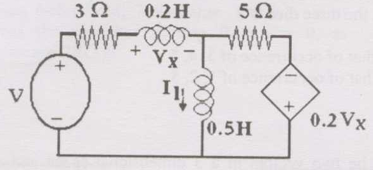
\includegraphics[width=0.45\linewidth]{figs/Q 50 2007.png} \caption{}     \label{fig:myfigure}
\end{figure}

\begin{enumerate}
   \item   $\dfrac{dI_1}{dt} = -1.4 V_x - 3.75 I_1 + \dfrac{5}{4} V$ 
\item  $\dfrac{dI_1}{dt} = 1.4 V_x - 3.75 I_1 - \dfrac{5}{4} V$
\item $\dfrac{dI_1}{dt} = -1.4 V_x + 3.75 I_1 + \dfrac{5}{4} V$
\item $\dfrac{dI_1}{dt} = -1.4 V_x + 3.75 I_1 - \dfrac{5}{4} V$

\end{enumerate}


\item \quad If $u(t)$, $r(t)$ denote the unit step and unit ramp functions respectively and $u(t)*r(t)$ their convolution, then the function $u(t+1)*r(t-2)$ is given by\hfill{(GATE EE 2007)} 

\begin{multicols}{4}
\begin{enumerate} 
\item (1/2)$(t-1)(t-2)$
\item (1/2)$(t-1)(t-2)$
\item (1/2)$(t-1)^2u(t-1)$
\item none of the above
\end{enumerate}
\end{multicols}

\item The integral
$
\frac{1}{2\pi}\int_0^{2\pi}\sin(t-\tau)\cos\tau\, d\tau
$
equals\hfill{(GATE EE 2007)} 

\begin{multicols}{4}
\begin{enumerate}
    \item $\sin t \cos t$
\item  $0$
\item  $(1/2) \cos t$
\item  $(1/2) \sin t$
\end{enumerate}
\end{multicols}

\vfill
\centering{EE 17/32}
\newpage


\item  \quad $X(z) = 1 - 3z^{-1}$,\quad $Y(z) = 1 + 2z^{-2}$ are Z-transforms of two signals $x[n],\,y[n]$ respectively.
A linear time invariant system has the impulse response $h[n]$ defined by these two signals as
$
    h[n] = x[n-1] * y[n]
$
where $*$ denotes discrete time convolution. Then the output of the system for the input $\delta[n-1]$\hfill{(GATE EE 2007)} 
\begin{enumerate}
    \item has Z-transform $z^{-1} X(z) Y(z)$
    \item equals $\delta[n-2] - 3\delta[n-3] + 2\delta[n-4] - 6\delta[n-5]$
    \item has Z-transform $1 - 3z^{-1} + 2z^{-2} - 6z^{-3}$
    \item does not satisfy any of the above three.
\end{enumerate}


\item  \quad A loaded dice has following probability distribution of occurrences

\begin{center}
\begin{tabular}{|c|c|c|c|c|c|c|}
\hline
Dice value      & 1   & 2   & 3   & 4   & 5   & 6   \\
\hline
Probability     & $1/4$ & $1/8$ & $1/8$ & $1/8$ & $1/8$ & $1/4$ \\
\hline
\end{tabular}
\end{center}

If three identical dice as the above are thrown, the probability of occurrence of values 1, 5 and 6 on the three dice is\hfill{(GATE EE 2007)} 
 
\begin{enumerate}
    \item same as that of occurrence of 3, 4, 5
    \item same as that of occurrence of 1, 2, 5
    \item$1/128$
    \item $5/8$
\end{enumerate}


\item  \quad Let $\vec{x}$ and $\vec{y}$ be two vectors in a 3 dimensional space and $\langle x, y \rangle$ denote their dot product.\\
Then the determinant
$
\det\myvec{
\langle x, x \rangle & \langle x, y \rangle \\
\langle y, x \rangle & \langle y, y \rangle 
}
$\hfill{(GATE EE 2007)} 
\noindent
\begin{enumerate}
\item is zero when $x$ and $y$ are linearly independent
\item is positive when $x$ and $y$ are linearly independent
\item is non-zero for all non-zero $x$ and $y$
\item is zero only when either $x$ or $y$ is zero
\end{enumerate}

\item  \quad The linear operation $\mathrm{L}(\vec{x})$ is defined by the cross product $\mathrm{L}(\vec{x}) = \vec{b} \times \vec{x}$, where $\vec{b} = [0\;1\;0]^T$ and $\vec{x} = [x_1\;x_2\;x_3]^T$ are three dimensional vectors. The $3 \times 3$ matrix $M$ of this operation satisfies
$
    \mathrm{L}(\vec{x}) = M \myvec{
        x_1 \\
        x_2 \\
        x_3
    }
$
Then the eigenvalues of $M$ are\hfill{(GATE EE 2007)} 

\begin{enumerate}
    \item $0$, $+1$, $-1$
    \item $1$, $-1$, $1$
    \item $i$, $-i$, $1$
    \item $i$, $-i$, $0$
\end{enumerate}

\vfill
\centering{EE 18/32}
\newpage

\item  \quad In the figure, transformer $T_1$ has two secondaries, all three windings having the same number of turns and with polarities as indicated. One secondary is shorted by a $10\,\Omega$ resistor $R$, and the other by a 15 $\mu$F capacitor. The switch SW is opened ($t=0$) when the capacitor is charged to 5V with the left plate as positive. At $t=0+$ the voltage $V_p$ and current $I_R$ are
\hfill{(GATE EE 2007)} 

\begin{figure}[H]
    \centering
    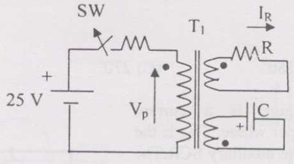
\includegraphics[width=0.5\linewidth]{figs/Q 57 2007.png} \caption{}     \label{fig:myfigure}
\end{figure}

\begin{multicols}{2}
\begin{enumerate}
\item  -$25$V,$0.0$ 
\item  very large voltage, very large current
\item   $5.0$V, $0.5$
\item  -$5.0$V ,-$0.5$ A
\end{enumerate}
\end{multicols}
\vspace{0.5cm}
\item  \quad IC 555 in the adjacent figure is configured as an astable multivibrator. It is enabled to oscillate at $t=0$ by applying a high input to pin 4. The pin description is: 1 and 8 -- supply; 2--trigger; 4--reset; 6--threshold; 7--discharge. The waveform appearing across the capacitor starting from $t=0$, as observed on a storage CRO is\hfill{(GATE EE 2007)} 
\begin{figure}[H]
    \centering
    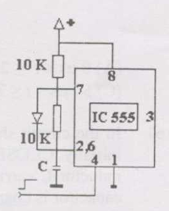
\includegraphics[width=0.2\linewidth]{figs/Q 58(Q).png} \caption{}     \label{fig:myfigure}
\end{figure}

\begin{figure}[H]
    \centering
    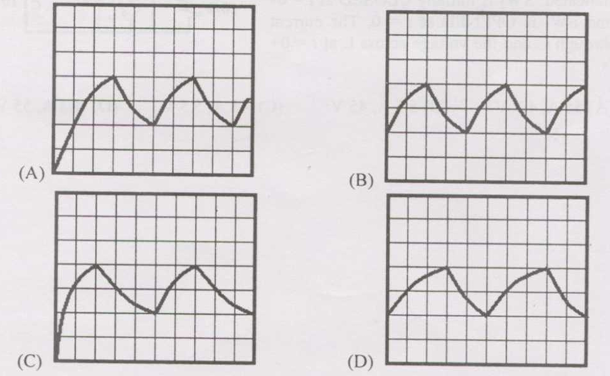
\includegraphics[width=0.5\linewidth]{figs/Q 58 opt.png} 
\end{figure}
\vfill
\centering{EE 19/32}
\newpage

\item  \quad In the circuit of adjacent figure the diode connects the ac
source to a pure inductance L.
\begin{figure}[H]
    \centering
    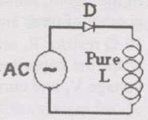
\includegraphics[width=0.2\linewidth]{figs/Q 59.png} \caption{}     \label{fig:myfigure}
\end{figure}


The diode conducts for\hfill{(GATE EE 2007)} 
\begin{multicols}{4}
\begin{enumerate}
\item The angle is $90^\circ$
\item $180^\circ$
\item $270^\circ$
\item $360^\circ$
\end{enumerate}
\end{multicols}

\item \quad The circuit in the figure is a current commutated dc--dc chopper where, $Th_{M}$ is the main SCR and $Th_{AUX}$  is the auxiliary SCR. The load current is constant at $10$ A. $Th_{M}$  is ON. $Th_{AUX}$  is triggered at $t=0$. $Th_{M}$  is turned OFF between\hfill{(GATE EE 2007)} 

\begin{figure}[H]
    \centering
    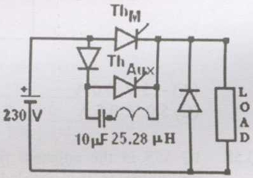
\includegraphics[width=0.45\linewidth]{figs/Q 60.png} \caption{}     \label{fig:myfigure}
\end{figure}


\begin{multicols}{2}
(A) $0~\mu\mathrm{s} < t \leq 25~\mu\mathrm{s}$ \\
(B) $25~\mu\mathrm{s} < t \leq 50~\mu\mathrm{s}$ \\
(C) $50~\mu\mathrm{s} < t \leq 75~\mu\mathrm{s}$ \\
(D) $75~\mu\mathrm{s} < t \leq 100~\mu\mathrm{s}$ \\
\end{multicols}

\item  \quad In the circuit shown in figure, switch SW$_1$ is initially CLOSED and SW$_2$ is OPEN. The inductor $L$ carries a current of $10~\mathrm{A}$ and the capacitor is charged to $10~\mathrm{V}$ with polarities as indicated. SW$_2$ is initially CLOSED at $t = 0-$ and SW$_1$ is OPENED at $t = 0$. The current through $C$ and the voltage across $L$ at $t = 0+$ is\hfill{(GATE EE 2007)} 

\begin{figure}[H]
    \centering
    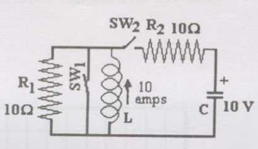
\includegraphics[width=0.3\linewidth]{figs/Q 61.png} \caption{}     \label{fig:myfigure}
\end{figure}


\begin{multicols}{4}
\begin{enumerate}
\item $55$A, $4.5$V
\item $5.5$A, $45$V
\item  $45$A, $5.5$V
\item $4.5$A, $55$V
\end{enumerate}
\end{multicols}

\vfill
\centering{EE 20/32}
\newpage
\item  \quad The R-L-C series circuit shown is supplied from a variable frequency voltage source. The admittance-locus of the R-L-C network at terminals AB for increasing frequency $\omega$ is\hfill{(GATE EE 2007)} 

\begin{figure}[H]
    \centering
    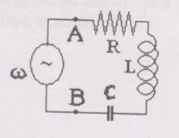
\includegraphics[width=0.3\linewidth]{figs/Q 62 Q.png} \caption{}     \label{fig:myfigure}
\end{figure}
    \begin{figure}[H]
    \centering
    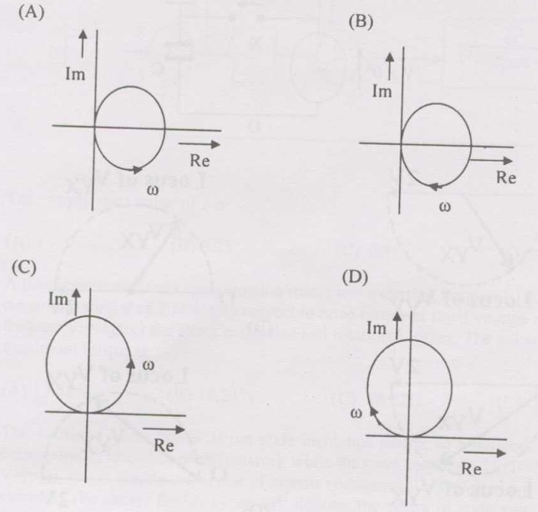
\includegraphics[width=0.85\linewidth]{figs/Q 62.png} 

\end{figure}
\vfill
\centering{EE 21/32}
\newpage
\item \quad In the figure given below all phasors are with reference to the potential at point ``O''. The locus of voltage phasor $V_{YX}$ as R is varied from zero to infinity is shown by\hfill{(GATE EE 2007)} 

\begin{figure}[H]
    \centering
    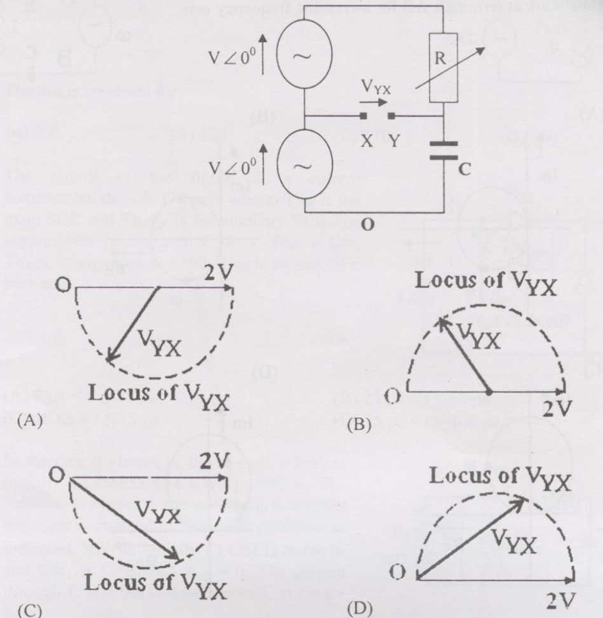
\includegraphics[width=1\linewidth]{figs/Q 63.png} \caption{}     \label{fig:myfigure}
\end{figure}
\vspace{1cm}
\item  \quad A 3V dc supply with an internal resistance of $2~\Omega$ supplies a passive non-linear resistance characterized by the relation $V_{NL} = I_{NL}^2$. The power dissipated in the non-linear resistance is\hfill{(GATE EE 2007)} 

\begin{multicols}{4}
\begin{enumerate}
    \item $1.0$  
\item $1.5$ 
\item $2.5$ 
\item $3.0$ 
\end{enumerate}
\end{multicols}

\vfill
\centering{EE 22/32}
\newpage

\item  \hspace{0.5em} \parbox[t]{0.85\textwidth}{%
Consider the feedback control system shown below which is subjected to a unit step input. The system is stable and has the following parameters $k_p = 4$, $k_i = 10$, $\omega = 500$ and $\xi = 0.7$.
} 

\begin{figure}[H]
    \centering
    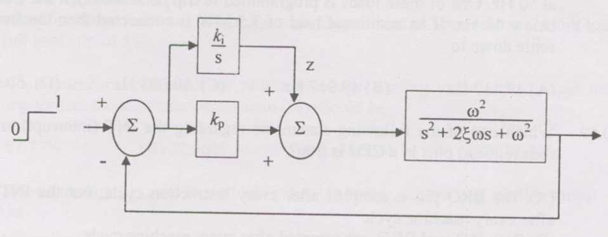
\includegraphics[width=0.7\linewidth]{figs/Q 65.png} \caption{}     \label{fig:myfigure}
\end{figure}

The steady state value of  is\hfill{(GATE EE 2007)}
\begin{multicols}{4}
\begin{enumerate}
\item $1$  
\item $0.25$  
\item $0.1$  
\item $0$  
 \end{enumerate}
\end{multicols}

\item  A three-phase squirrel cage induction motor has a starting torque of 150\% and a maximum torque of 300\% with respect to rated torque at rated voltage and rated frequency. Neglect the stator resistance and rotational losses. The value of slip for maximum torque is\hfill{(GATE EE 2007)}

\begin{multicols}{4}
\begin{enumerate}
\item  13.48\% 
\item 16.24\% 
\item 18.92\% 
\item 26.79\%
\end{enumerate}
\end{multicols}

\vspace{1em}
\item  
The matrix $A$ given below is the node incidence matrix of a network. The columns correspond to branches of the network while the rows correspond to nodes. Let $\vec{V} = [v_1\, v_2\, \ldots\, v_6]^T$ denote the vector of branch voltages while $\vec{I} = [i_1\, i_2\, \ldots\, i_6]^T$ that of branch currents. The vector $\vec{E} = [e_1\, e_2\, e_3\, e_4]^T$ denotes the vector of node voltages relative to a common ground.
$
A =
\myvec{
1 & 1 & 1 & 0 & 0 & 0 \\
0 & -1 & 0 & -1 & 1 & 0 \\
-1 & 0 & 0 & 0 & -1 & -1 \\
0 & 0 & -1 & 1 & 0 & 1 \\
}
$
Which of the following statements is true?\hfill{(GATE EE 2007)}
\begin{enumerate}
    \item[(A)] The equations\\
        \hspace*{1.5em}$v_1 - v_2 + v_3 = 0$, \ $v_3 + v_4 - v_5 = 0$\\
        are KVL equations for the network for some loops
    \item[(B)] The equations\\
        \hspace*{1.5em}$v_1 - v_3 - v_6 = 0$, \ $v_4 + v_5 - v_6 = 0$\\
        are KVL equations for the network for some loops
    \item[(C)] $\vec{E} = A\vec{V}$
    \item[(D)] $A\vec{V} = 0$ are KVL equations for the network
\end{enumerate}

\vfill
\centering{EE 23/32}
\newpage

\item  
An isolated 50 Hz synchronous generator is rated at 15 MW which is also the maximum continuous power limit of its prime mover. It is equipped with a speed governor with 5\% droop. Initially, the generator is feeding three loads of 4 MW each at 50 Hz. One of these loads is programmed to trip \textit{permanently} if the frequency falls below 48 Hz. If an additional load of 3.5 MW is connected then the frequency will settle down to\hfill{(GATE EE 2007)}

\begin{multicols}{4}
\begin{enumerate}
\item  49.417 Hz
\item  49.917 Hz
\item  50.083 Hz
\item  50.583 Hz
\end{enumerate}
\end{multicols}

\vspace{1em}

\item 
Which one of the following statements regarding the INT (interrupt) and the BRQ (bus request) pins in a CPU is true?\hfill{(GATE EE 2007)}

\begin{enumerate}
    \item[(A)] The BRQ pin is sampled after every instruction cycle, but the INT is sampled after every machine cycle
    \item[(B)] Both INT and BRQ are sampled after every machine cycle
    \item[(C)] The INT pin is sampled after every instruction cycle, but the BRQ is sampled after every machine cycle
    \item[(D)] Both INT and BRQ are sampled after every instruction cycle
\end{enumerate}

\vspace{1em}

\item 
A bridge circuit is shown in the figure below. Which one of the sequences given below is most suitable for balancing the bridge?\hfill{(GATE EE 2007)}

\begin{figure}[H]
    \centering
    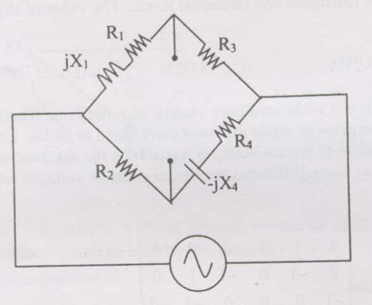
\includegraphics[width=0.5\linewidth]{figs/Q 70.png} \caption{}     \label{fig:myfigure}
\end{figure}

\begin{multicols}{2}
\begin{enumerate}
 \item  First adjust $R_4$, and then adjust $R_1$
\item   First adjust $R_2$, and then adjust $R_3$
 \item   First adjust $R_2$, and then adjust $R_4$
 \item  First adjust $R_4$, and then adjust $R_2$
 \end{enumerate}
\end{multicols}

\vfill
\centering{EE 24/32}
\newpage

\textbf{Common Data Questions}\\

\vspace{1cm}

\raggedright{\textbf{Common Data for Questions 71,72,73:}}

A three phase squirrel cage induction motor has a starting current of seven times the full load current and full load slip of 5\%.

\vspace{1em}

\item   If an autotransformer is used for reduced voltage starting to provide 1.5 per unit starting torque, the autotransformer ratio (\%) should be\hfill{(GATE EE 2007)}

\begin{multicols}{4}
\begin{enumerate}
\item  57.77\% 
\item  72.56\% 
\item  78.25\% 
\item  81.33\%
\end{enumerate}
\end{multicols}

\vspace{0.5em}

\item   If a star-delta starter is used to start this induction motor, the per unit starting torque will be\hfill{(GATE EE 2007)}

\begin{multicols}{4}
\begin{enumerate}
    \item  0.607
 \item  0.816
 \item  1.225
 \item  1.616
\end{enumerate}
\end{multicols}

\vspace{0.5em}

\item If a starting torque of 0.5 per unit is required then the per unit starting current should be\hfill{(GATE EE 2007)}

\begin{multicols}{4}
\begin{enumerate}
\item 4.65 
\item 3.75 
\item 3.16 
\item 2.13 
\end{enumerate}
\end{multicols}

\vspace{1em}

\noindent\textbf{Common Data for Questions 74, 75:}

A 1:1 Pulse Transformer (PT) is used to trigger the SCR in the adjacent figure. The SCR is rated at 1.5 kV, 250 A with $I_L = 250$ mA, $I_H = 150$ mA, and $I_{Gmax} = 150$ mA, $I_{Gmin} = 100$ mA. The SCR is connected to an inductive load, where $L = 150$ mH in series with a small resistance and the supply voltage is 200V dc. The forward drops of all transistors/diodes and gate-cathode junction during ON state are 1.0 V.


\begin{figure}[H]
    \centering
    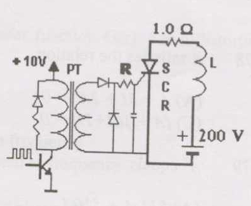
\includegraphics[width=0.4\linewidth]{figs/Q 74,75,76.png} \caption{}     \label{fig:myfigure}
\end{figure}

\begin{minipage}{0.6\textwidth}
\item  The resistance R should be\hfill{(GATE EE 2007)}
\begin{multicols}{4}
\begin{enumerate}
    \item  4.7 k$\Omega$ 
 \item  470 $\Omega$
 \item  47 $\Omega$ 
 \item  4.7 $\Omega$ 
\end{enumerate}
\end{multicols}

\item  The minimum approximate volt-second rating of the pulse transformer suitable for triggering the SCR should be: (volt–second rating is the maximum of product of the voltage and the width of the pulse that may be applied)\hfill{(GATE EE 2007)}
\begin{multicols}{4}
\begin{enumerate}
   \item  2000 $\mu$V-s
 \item  200 $\mu$V-s
 \item  20 $\mu$V-s 
 \item  2.0 $\mu$V-s 
\end{enumerate}
\end{multicols}
\end{minipage}
\hfill

\vfill
\centering{EE 25/32}
\newpage

{\textbf{Linked Answer Questions:Q.76 to Q.85 carry two marks each.}}
\vspace{0.5cm}

\raggedright{\textbf{Statement for Linked Answer Questions 76 \& 77:}}

\noindent

An inductor designed with 400 turns coil wound on an iron core of 16 cm$^2$ cross sectional area \\
and with a cut of an air gap length of 1 mm. The coil is connected to a 230 V, 50 Hz ac \\
supply. Neglect coil resistance, core loss, iron reluctance and leakage inductance. ($\mu_0 = 4\pi \times 10^{-7}$ H/m)

\vspace{1em}

\item  The current in the inductor is\hfill{(GATE EE 2007)}

\begin{multicols}{4}
\begin{enumerate}
    \item  18.08 A 
\item  9.04 A
\item  4.56 A 
\item 2.28 A 
\end{enumerate}
\end{multicols}

\item  The average force on the core to reduce the air gap will be\hfill{(GATE EE 2007)}

\begin{multicols}{4}
\begin{enumerate}
    \item  832.29 N 
\item  1666.22 N 
\item  3332.47 N 
\item  6664.84 N 
\end{enumerate}
\end{multicols}

\vspace{1em}

\noindent
\textbf{Statement for Linked Answer Questions 78 \& 79:} \\
Cayley-Hamilton Theorem states that a square matrix satisfies its own characteristic equation. \\
Consider a matrix
$
A =
\myvec{
-3 & 2 \\
-1 & 0
}
$

\item  $A$ satisfies the relation\hfill{(GATE EE 2007)}

\begin{multicols}{2}
\begin{enumerate}
    \item  $A + 3I + 2A^{-1} = 0$ 
 \item  $A^2 + 2A + 3I = 0$
 \item  $(A + I)(A + 2I) = 0$ 
 \item  $\exp(A) = 0$ 
\end{enumerate}
\end{multicols}

\item  $A^9$ equals\hfill{(GATE EE 2007)}

\begin{multicols}{2}
\begin{enumerate}
\item $511\, A + 510\, I$
\item $309\, A + 104\, I$
\item $154\, A + 155\, I$
\item $\exp(9A)$ 
\end{enumerate}
\end{multicols}

\noindent
\textbf{Statement for Linked Answer Questions 80 \& 81:}\\
Consider the R-L-C circuit shown in figure.
\begin{figure}[H]
    \centering
    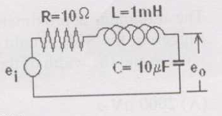
\includegraphics[width=0.3\linewidth]{figs/Q 80,81.png} \caption{}     \label{fig:myfigure}
\end{figure}
\item  For a step-input $e_i$, the overshoot in the output $e_o$ will be\hfill{(GATE EE 2007)}

\begin{multicols}{4}
\begin{enumerate}
    \item  0, since the system is not under-damped
  \item 5\% 
  \item  16\% 
  \item  48\% 
\end{enumerate}
\end{multicols}

\item  If the above step response is to be observed on a non-storage CRO, then it would be best to have the $e_i$ as a\hfill{(GATE EE 2007)}

\begin{multicols}{2}
\begin{enumerate}
 \item  step function 
\item square wave of frequency 50 Hz 
\item  square wave of frequency 300 Hz 
\item  square wave of frequency 2.0 kHz
\end{enumerate}
\end{multicols}
\newpage
\noindent
\textbf{Statement for Linked Answer Questions 82 \& 83:}\\
The associated figure shows the two types of rotate right instructions R1, R2 available in a microprocessor where Reg is a 8-bit register and C is the carry bit. The rotate left instructions L1 and L2 are similar except that C now links the most significant bit of Reg instead of the least significant one.

\vspace{0.5em}

\begin{figure}[H]
    \centering
    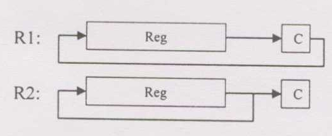
\includegraphics[width=0.5\linewidth]{figs/Q 82,83.png} \caption{}     \label{fig:myfigure}
\end{figure}

\item 
Suppose Reg contains the 2's complement number 11010110. If this number is divided by 2 the answer should be\hfill{(GATE EE 2007)}

\begin{multicols}{4}
\begin{enumerate}
    \item  01101011 
 \item  10010101 
 \item  11101001 
 \item  11101011 
\end{enumerate}
\end{multicols}
\item  Such a division can be correctly performed by the following set of operations\hfill{(GATE EE 2007)}

\begin{multicols}{4}
\begin{enumerate}
   \item  L2, R2, R1 
  \item  L2, R1, R2 
  \item  R2, L1, R1 
  \item  R1, L2, R2
\end{enumerate}
\end{multicols}

\vspace{1em}

\noindent
\textbf{Statement for Linked Answer Questions 84 \& 85:}\\
\item A signal is processed by a causal filter with transfer function $G(s)$. For a distortion free output signal waveform, $G(s)$ must\hfill{(GATE EE 2007)}

\begin{enumerate}
\item[(A)] provide zero phase shift for all frequency
\item[(B)] provide constant phase shift for all frequency
\item[(C)] provide linear phase shift that is proportional to frequency
\item[(D)] provide a phase shift that is inversely proportional to frequency
\end{enumerate}

\item 
$G(z) = \alpha z^{-1} + \beta z^{-3}$ is a low-pass digital filter with a phase characteristics same as that of the above question if
\hfill{(GATE EE 2007)}
\begin{multicols}{4}
\begin{enumerate}
  \item  $\alpha = \beta$ 
\item  $\alpha = -\beta$
\item  $\alpha = \beta^{(1/3)}$ 
\item  $\alpha = \beta^{-(1/3)}$  
\end{enumerate}
\end{multicols}

\vskip 2em

\textbf{END OF THE QUESTION PAPER}
\vfill
\centering{EE 27/32}


\end{enumerate}
\end{document}

\caption{}
    \label{fig:myfigure}